\section{Investigating narratives and storytelling with Klimahuset}
\par
\emph{31.05.2021, narrative workshop with Klimahuset}
\par

Inspired by Emilie Sitzia’s exploration of narrative theories and learning in contemporary art museums, and the way narratives are constructed in a museum context, me and my research buddies looked into how narratives play a part in telling a story and in conveying a message. Some of the thoughts behind the first workshop we had in April with stakeholders from Klimahuset, was that we wanted to explore how to engage participants in building a narrative. By inviting stakeholders from Klimahuset, we anticipated that we would get a better understanding on how to build up climate crisis related narratives. This would also give us the opportunity to get some input on which sustainability issues can be a better fit, topic-wise, when designing for a learning-oriented type of installation. We also wanted to facilitate a conversation on the current existing exhibition in Klimahuset, to get some feeling if there were any topics or sustainability issues they wish the current exhibition should address.

The workshop in itself consisted of three phases; brainstorming, storyboarding and presentation phase. It was conducted digitally through zoom, using Miro as the workshop platform-tool. We primarily wanted to get a better grip on different topics and issues in the climate debate that could be used as groundwork for design fictions, which is why we tried to brainstorm three dimensions that can make up a story; a theme, an dilemma and a setting. Therefore we asked them:
What topics in the climate debate do you think is important to address?
Write down issues/ dilemmas related to climate debates.
Write down (a climate-related) setting.
In the next part of the workshop we wanted the participants to create their own individual storyboard, where they could choose between all commonly brainstormed themes, dilemmas and settings - to make up their own story that they would later present. And then to finalise the workshop, the participants one by one presented their story. It was interesting to see the diversity and different perspectives from the participants and their respective stories. Even though some participants had used the same theme, dilemma or setting, they all differed in terms of what the participant wanted to convey with their story. 

In the aftermath of this workshop, the collected stories and notes from the discussions have worked as a foundation for me to look into the relationship between narratives, dissemination in museums and meaning-making. The main finding I got from the workshop is the notion on how a well written narrative have the power to make us think about or see ourselves and the Earth around us with new eyes, enabling us to engage in and relate to the climate crisis through the narrative that is told. The climate crisis is first and foremost a story about humans and humanity, and the power in the narrative therefore lies in the message conveyed. 

\begin{figure}[h]
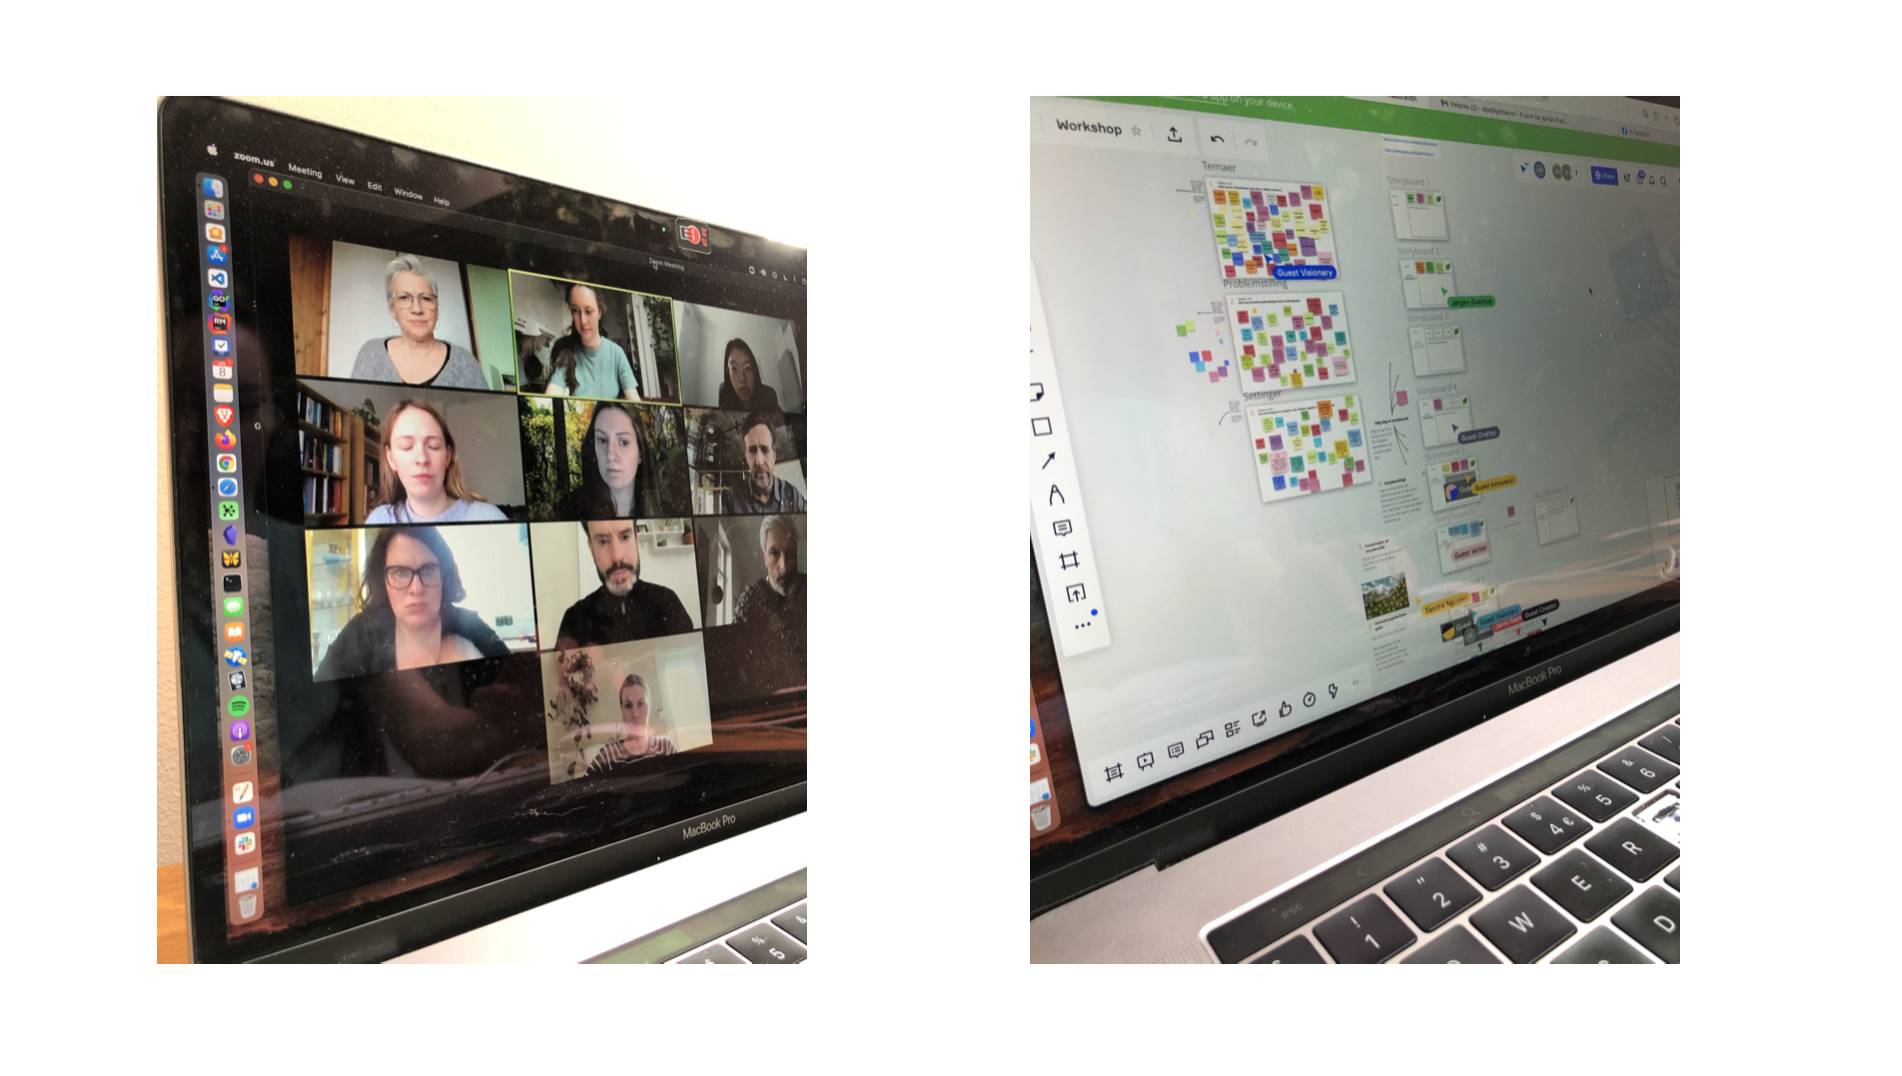
\includegraphics[width=13cm]{pictures/narrative_workshop.png}
\centering 
\end{figure}


\section{Observing Klimahusets narrative storytelling in-action}
\par
\emph{Observation and interview 16.02.2022}
\par

After my readings on the museum and its expository agency, I wonder what Klimahuset’s stakeholders thoughts are on their agency? And their position toward whether or not they have a subjective or objective expository agency? What are the cultural attitudes, decisions, views and stances the agents involved in designing the climate exhibition in Klimahuset, took before they decided to do the act of exposing? What cultural function does the objects on display in Klimahuset pose? 

Some of these questions can already kind of be elaborated for, from initial reading on internal documents that I have gotten access through collaborating partners in Klimahuset, as well as from conversations with stakeholders from Klimahuset last semester through the workshop, mail correspondence and mini-exhibition. As accounted for in Klimahusets founding documents, their vision/ purpose of the museum is as follows:
To give the visitors an understanding of the most important climate processes that affect the living conditions on Earth so that they are able to develop their own views on climate change, take part in climate discussions or act in other ways in relation to the topic.
Visitors must gain an understanding that natural conditions also affect social structures and culture.
	
Building on Mieke Bal’s narrative analysis on cultural imperialism in museums, say we look at Klimahuset as an ethnographic museum with the expository agency to display installations, objects and data related to the climate crisis. And with a distinct and clear target group being children aged 10-14. Is Klimahusets agency and vision an attempt to display the climate crisis as a current/ ongoing discourse with the function to educate and stimulate critical reflections on current societal norms and ways of living, or is the agency to define and lay up cultural change, to a more sustainable way of living? Maybe both? If so, then comes the question if the museums cultural stakeholders, with this expository agency, are they cultural moralists? Especially because their whole museum exhibition are designed to engage children aged 10-14, though welcoming all age groups, raises the question if the museum and exhibition design in itself potentially have any moral imperialistic function as well, as to who the discourse (the climate crisis) is relevant for. 
Asked the klimaverter about  this, need to do some structural analysis of some sort….

\begin{figure}[h]
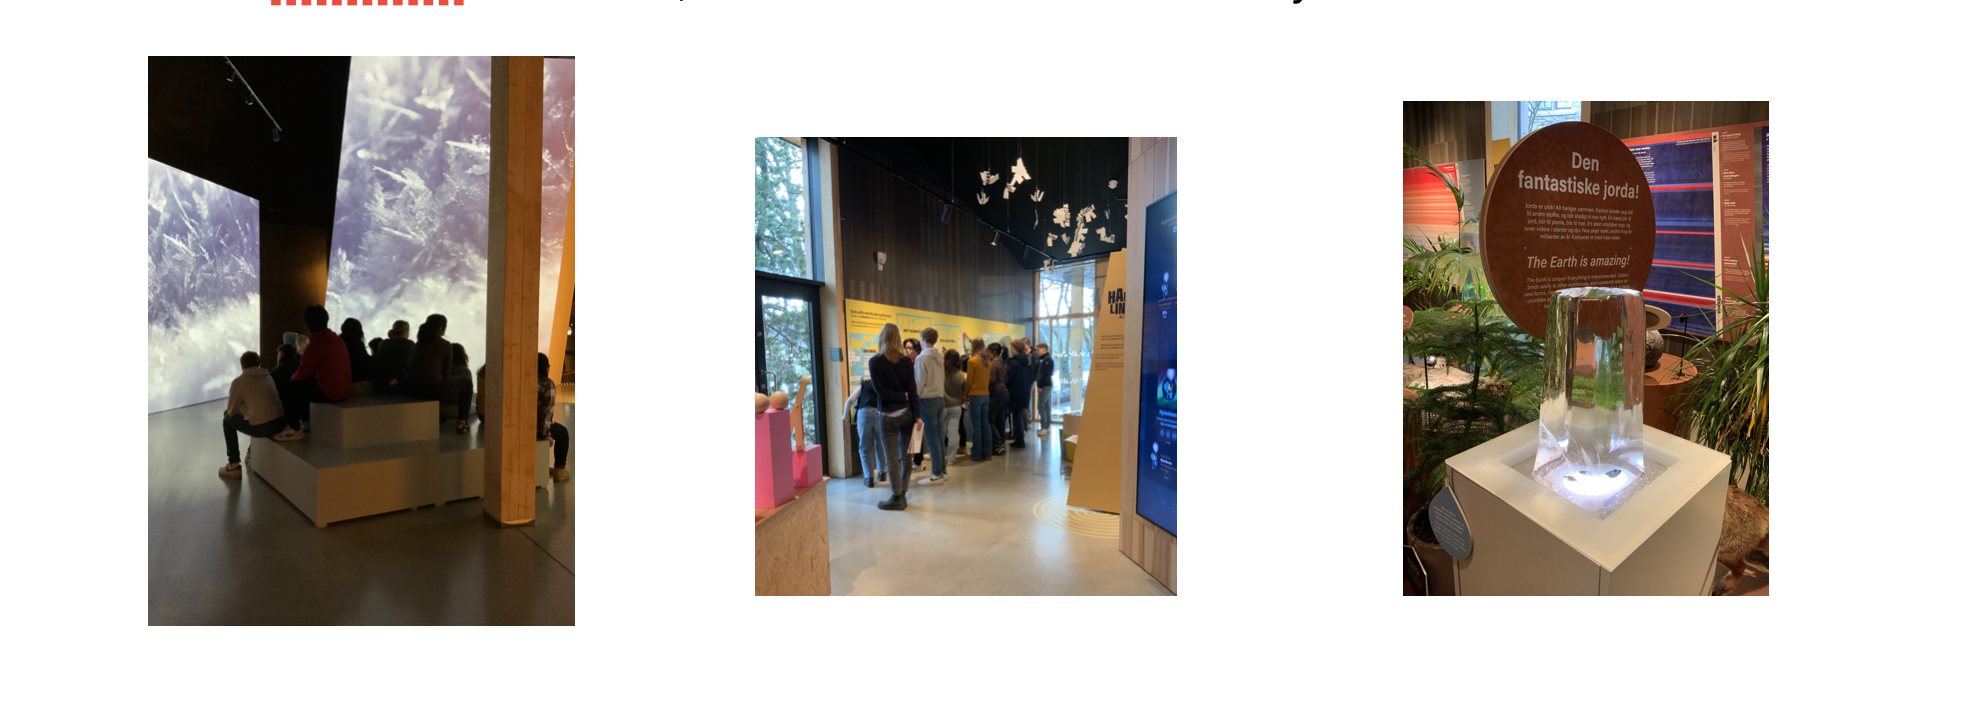
\includegraphics[width=13cm]{pictures/elever_i_klimahuset.png}
\centering 
\end{figure}

Med en klimavert til stede får man bedre hjelp og en form for retning til å “lese” installasjonene, som støtter deg når du senere går gjennom avdeling for avdeling. 
Man blir stilt spørsmål som er knyttet til faktiske ting, som for eksempel i video-atriet sier klimavert; jeg er 160cm høy, hvor høy tror dere denne veggen er?
Etter litt håndsopprekning får vi vite at dersom Grønlandsisen smelter vil havet stige like høyt som det den veggen er. Det er tankevekkende og setter inntrykk!

Her blir man også litt senere spurt: ser dere vær eller klima? et åpent spørsmål som setter i gang en god diskusjon på forskjellen mellom vær og klima, med fokus på hvordan vær påvirker klima. Dette blir forklart at mange blander og tenker at vær og klima er det samme, og at klimaforandringer og værforandringer ikke er det samme. Her får noen elever aha-øyeblikk.


Et annet eksempel er isbiten inne i “den naturlige avdelingen”.  Først får elevene i oppgave å finne noe i området som påvirker klimaet naturlig. Senere når det blir tatt en liten runde spør verten; har alle tatt på isbiten? For så å gå videre til å forklare hvordan menneskelig påvirkning påvirker klimaet. “For eksempel har deres varme hender bidratt til å smelte litt av isbiten her i Klimahuset”. Dette er også tankevekkende og setter inntrykk!


\section{Exploring input through plants}
\par
\emph{01.05.2021, presentation at Klimahuset}
\par

The thought behind this project was to explore how human touch on plants could be used as input, or as a type of controller, to manipulate elements of the installation. The statement of using an actual, living plant would be to reference the nature and its species: plants, animals and ecosystems, bringing the nature closer to the discourse where sustainability issues are discussed, inviting to reflections to the ecological damage that we are responsible for. I think this exploration addresses the research question as to how interactive artefacts can provide new depth to the museum discourse, by exploring how human touch through plants can stimulate emotions or values like empathy and awareness, reinforced by the educational environment (the whole museum) the installation is placed in. I believe the plant installation could be interesting to use in combination with learning about plant/ nature related climate disturbances like the burning and destroying of the rainforest, but also in a local, Norwegian context; the windmill debate, hydropower, national park borders, repercussions of cottage development or light pollution. During the shaping of this exploration, I managed to define yet a research question that I want to inquire into; can new/different interactions with natural objects contribute to increased climate consciousness and activism?	

\begin{figure}[H]
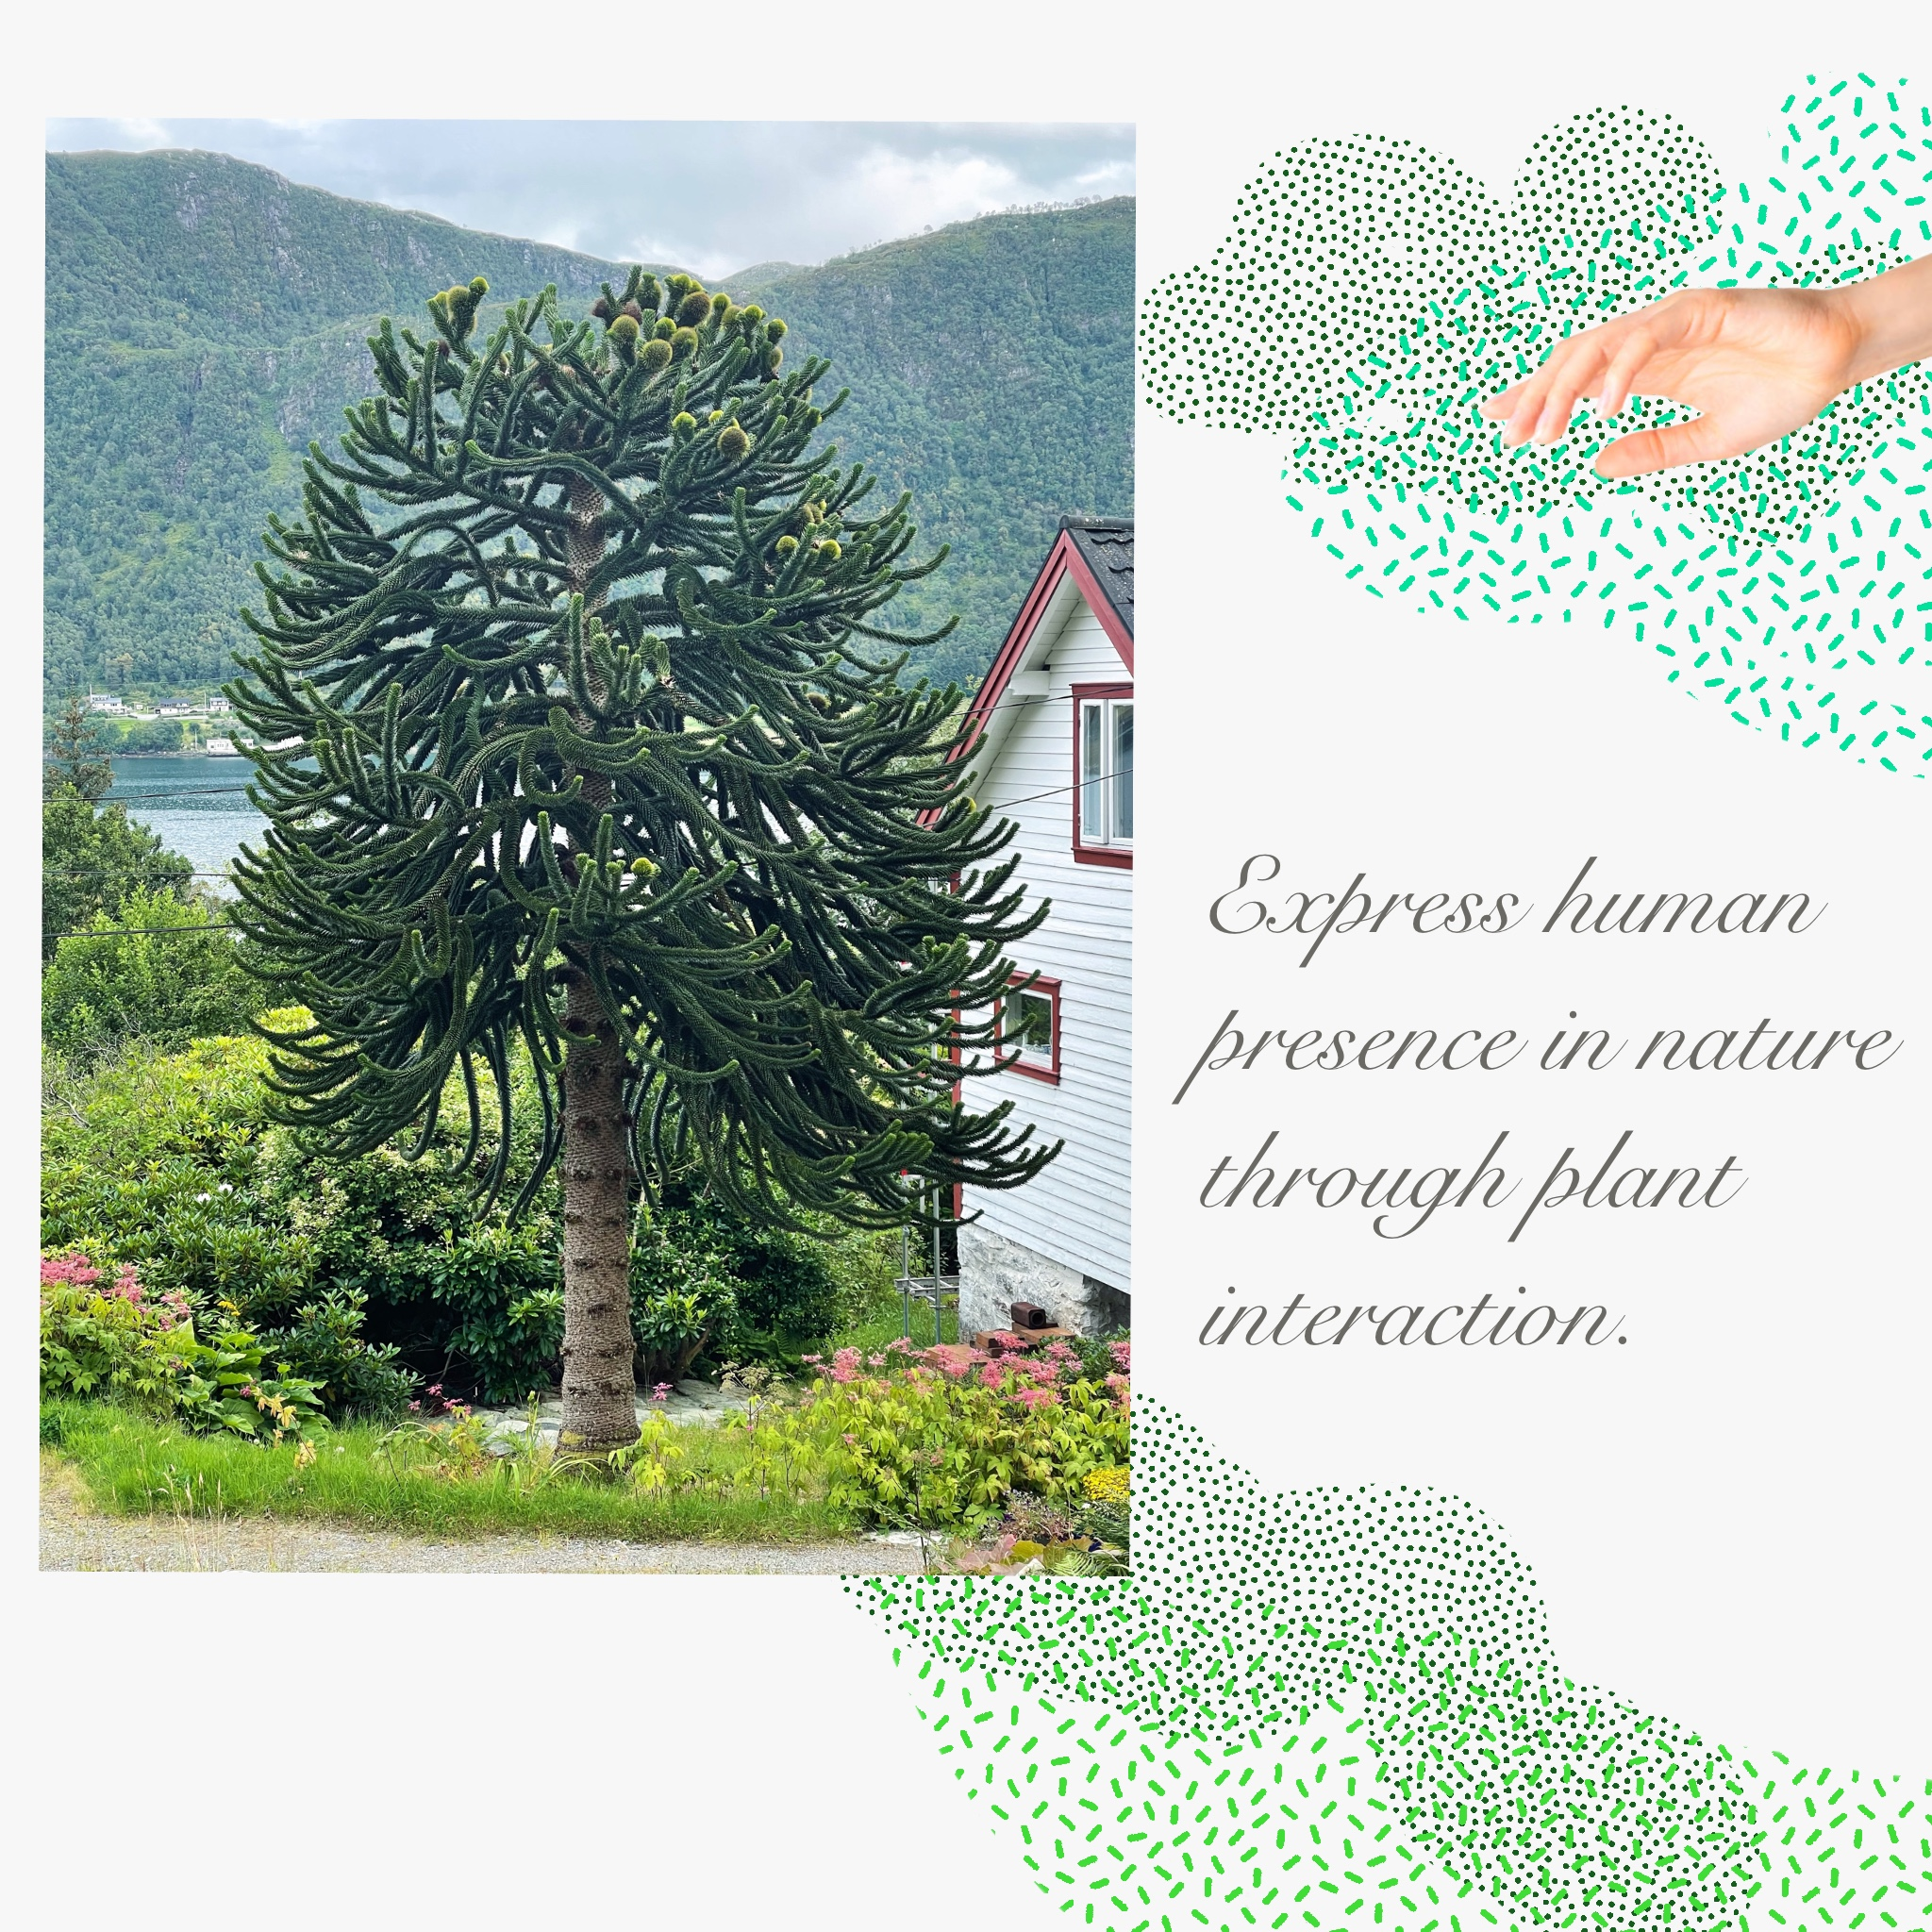
\includegraphics[width=10cm]{pictures/human_presence.jpg}
\centering 
\end{figure}


\section{Exhibition: Yuko Mohri}
\par
\emph{excursion to Atelier 21, dato xxx}
\par

example of a situated exhibition (place as dialogue),
which strategies and meaningful relations found place in the exhibition?


The physical qualities of the space:
Utstillingslokalet var et stort, tomt og åpent rom. Yuko Mohri sin utstilling besto av to installasjoner, hvorav de var plassert i sentrum av rommet/ spacet.  Det var også et lite avhjørne/ rom hvor man kunne ta på seg hodetelefoner og se en film som presenterte og beskrev verkene litt mer i dybden slik Yuko Mohri ville fortelle de.

Utstillingslokalet var ganske lite, og litt med gulvets materialitet og store åpne flater, samt relativt god takhøyde var det mye ekko når man gikk rundt. Jeg hadde på meg støvletter som “klakket” litt ekstra, og som ledet oppmerksomheten mot bevegelse i rommet. Effekten ble veldig forsterket etter at man hadde stått stille en stund også beveget enten du, eller noen andre i publikumet, seg, og da blir man dratt litt frem og tilbake mellom tilstedeværelsen i rommet og tilstedeværelsen knyttet til installasjonen. Lyden er i dialog med installasjonen. 
Jeg noterte meg også at i dette litt mindre spacet, får man lettere øyekontakt med de andre besøkende, og at man ble litt ekstra vár de andres tilstedeværelse. Litt kleint å snakke høyt, man vet at alle hører hva du sier.

\begin{figure}[H]
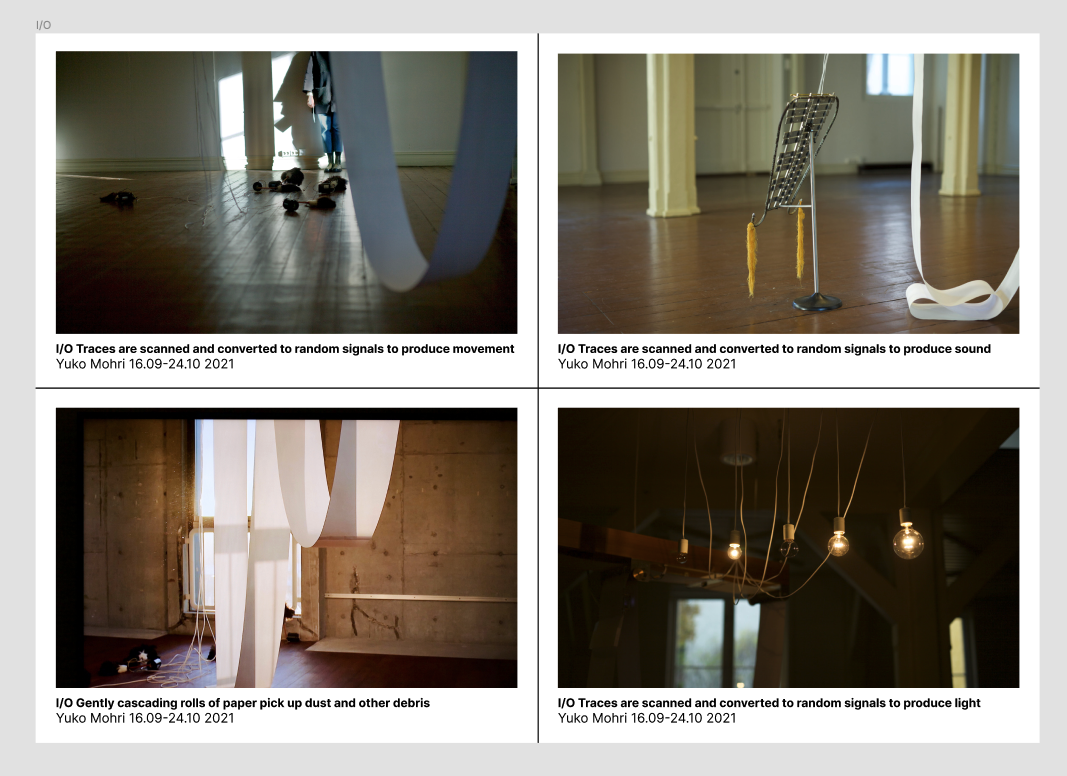
\includegraphics[width=15cm]{pictures/yukomohri.png}
\centering 
\end{figure}

\section{Exhibition: Munch museum}
\par
\emph{27.10.2021, excursion to Munch Museum w/ focus on the interactive Poison exhibition.}
\par

Munch is a great example of how they use text and plaques to inform/guide the visitor in terms of how they can read some of the art they see. It is a good example of how one can design the visitor journey through the exhibition space. It supports the visitors sense-making, in terms of how they can use and move through the space. However, it is an analogous way to support sense-making, while I am interested in ways interactivity can support this type of sense-making. Even in the interactive Poison exhibition, the information is static.

\begin{figure}[h]
\includegraphics[width=13cm]{pictures/pink_munch.jpeg}
\centering 
\end{figure}

\section{Interview with a concept developer from Munch}
\par
\emph{date date date}
\par

